% test
% Template for PLoS
% Version 3.5 March 2018
%
% % % % % % % % % % % % % % % % % % % % % %
%
% -- IMPORTANT NOTE
%
% This template contains comments intended
% to minimize problems and delays during our production
% process. Please follow the template instructions
% whenever possible.
%
% % % % % % % % % % % % % % % % % % % % % % %
%
% Once your paper is accepted for publication,
% PLEASE REMOVE ALL TRACKED CHANGES in this file
% and leave only the final text of your manuscript.
% PLOS recommends the use of latexdiff to track changes during review, as this will help to maintain a clean tex file.
% Visit https://www.ctan.org/pkg/latexdiff?lang=en for info or contact us at latex@plos.org.
%
%
% There are no restrictions on package use within the LaTeX files except that
% no packages listed in the template may be deleted.
%
% Please do not include colors or graphics in the text.
%
% The manuscript LaTeX source should be contained within a single file (do not use \input, \externaldocument, or similar commands).
%
% % % % % % % % % % % % % % % % % % % % % % %
%
% -- FIGURES AND TABLES
%
% Please include tables/figure captions directly after the paragraph where they are first cited in the text.
%
% DO NOT INCLUDE GRAPHICS IN YOUR MANUSCRIPT
% - Figures should be uploaded separately from your manuscript file.
% - Figures generated using LaTeX should be extracted and removed from the PDF before submission.
% - Figures containing multiple panels/subfigures must be combined into one image file before submission.
% For figure citations, please use "Fig" instead of "Figure".
% See http://journals.plos.org/plosone/s/figures for PLOS figure guidelines.
%
% Tables should be cell-based and may not contain:
% - spacing/line breaks within cells to alter layout or alignment
% - do not nest tabular environments (no tabular environments within tabular environments)
% - no graphics or colored text (cell background color/shading OK)
% See http://journals.plos.org/plosone/s/tables for table guidelines.
%
% For tables that exceed the width of the text column, use the adjustwidth environment as illustrated in the example table in text below.
%
% % % % % % % % % % % % % % % % % % % % % % % %
%
% -- EQUATIONS, MATH SYMBOLS, SUBSCRIPTS, AND SUPERSCRIPTS
%
% IMPORTANT
% Below are a few tips to help format your equations and other special characters according to our specifications. For more tips to help reduce the possibility of formatting errors during conversion, please see our LaTeX guidelines at http://journals.plos.org/plosone/s/latex
%
% For inline equations, please be sure to include all portions of an equation in the math environment.  For example, x$^2$ is incorrect; this should be formatted as $x^2$ (or $\mathrm{x}^2$ if the romanized font is desired).
%
% Do not include text that is not math in the math environment. For example, CO2 should be written as CO\textsubscript{2} instead of CO$_2$.
%
% Please add line breaks to long display equations when possible in order to fit size of the column.
%
% For inline equations, please do not include punctuation (commas, etc) within the math environment unless this is part of the equation.
%
% When adding superscript or subscripts outside of brackets/braces, please group using {}.  For example, change "[U(D,E,\gamma)]^2" to "{[U(D,E,\gamma)]}^2".
%
% Do not use \cal for caligraphic font.  Instead, use \mathcal{}
%
% % % % % % % % % % % % % % % % % % % % % % % %
%
% Please contact latex@plos.org with any questions.
%
% % % % % % % % % % % % % % % % % % % % % % % %

\documentclass[10pt,letterpaper]{article}
\usepackage[top=0.85in,left=2.75in,footskip=0.75in]{geometry}

% amsmath and amssymb packages, useful for mathematical formulas and symbols
\usepackage{amsmath,amssymb}

% Use adjustwidth environment to exceed column width (see example table in text)
\usepackage{changepage}

% Use Unicode characters when possible
\usepackage[utf8x]{inputenc}

% textcomp package and marvosym package for additional characters
\usepackage{textcomp,marvosym}

% cite package, to clean up citations in the main text. Do not remove.
\usepackage{cite}

% Use nameref to cite supporting information files (see Supporting Information section for more info)
\usepackage{nameref,hyperref}

% line numbers
\usepackage[right]{lineno}

% ligatures disabled
\usepackage{microtype}
\DisableLigatures[f]{encoding = *, family = * }

% color can be used to apply background shading to table cells only
\usepackage[table]{xcolor}

% array package and thick rules for tables
\usepackage{array}

% create "+" rule type for thick vertical lines
\newcolumntype{+}{!{\vrule width 2pt}}

% create \thickcline for thick horizontal lines of variable length
\newlength\savedwidth
\newcommand\thickcline[1]{%
  \noalign{\global\savedwidth\arrayrulewidth\global\arrayrulewidth 2pt}%
  \cline{#1}%
  \noalign{\vskip\arrayrulewidth}%
  \noalign{\global\arrayrulewidth\savedwidth}%
}

% \thickhline command for thick horizontal lines that span the table
\newcommand\thickhline{\noalign{\global\savedwidth\arrayrulewidth\global\arrayrulewidth 2pt}%
\hline
\noalign{\global\arrayrulewidth\savedwidth}}


% Remove comment for double spacing
%\usepackage{setspace}
%\doublespacing

% Text layout
\raggedright
\setlength{\parindent}{0.5cm}
\textwidth 5.25in
\textheight 8.75in

% Bold the 'Figure #' in the caption and separate it from the title/caption with a period
% Captions will be left justified
\usepackage[aboveskip=1pt,labelfont=bf,labelsep=period,justification=raggedright,singlelinecheck=off]{caption}
\renewcommand{\figurename}{Fig}

% Use the PLoS provided BiBTeX style
\bibliographystyle{plos2015}

% Remove brackets from numbering in List of References
\makeatletter
\renewcommand{\@biblabel}[1]{\quad#1.}
\makeatother



% Header and Footer with logo
\usepackage{lastpage,fancyhdr,graphicx}
\usepackage{epstopdf}
%\pagestyle{myheadings}
\pagestyle{fancy}
\fancyhf{}
%\setlength{\headheight}{27.023pt}
%\lhead{\includegraphics[width=2.0in]{PLOS-submission.eps}}
\rfoot{\thepage/\pageref{LastPage}}
\renewcommand{\headrulewidth}{0pt}
\renewcommand{\footrule}{\hrule height 2pt \vspace{2mm}}
\fancyheadoffset[L]{2.25in}
\fancyfootoffset[L]{2.25in}
\lfoot{\today}

%% Include all macros below

\newcommand{\lorem}{{\bf LOREM}}
\newcommand{\ipsum}{{\bf IPSUM}}

%% END MACROS SECTION


\begin{document}
\vspace*{0.2in}

% Title must be 250 characters or less.
\begin{flushleft}
{\Large
\textbf\newline{Instantaneous Reproduction Number Estimation From Modelled Incidence}
}
\newline
% Insert author names, affiliations and corresponding author email (do not include titles, positions, or degrees).
\\
Robert Challen\textsuperscript{1,2*},
Leon Danon\textsuperscript{1,2}
\\
\bigskip
\textbf{1} AI4CI, University of Bristol, Bristol, UK.\\
\textbf{2} Department of Engineering Mathematics, University of Bristol, Bristol, UK.\\
\bigskip

% Insert additional author notes using the symbols described below. Insert symbol callouts after author names as necessary.
% Use the asterisk to denote corresponding authorship and provide email address in note below.
* rob.challen@bristol.ac.uk

\end{flushleft}
% Please keep the abstract below 300 words
\section*{Abstract}

The time-varying reproduction number ($R_t$) is a critical quantity in monitoring an infectious disease outbreak. We propose a new method for estimating $R_t$ from an infectivity profile, expressed as a generation time distribution, and a time series of probabilistic estimates of disease incidence, modelled as log-normally distributed random variables. This is a common output of disease incidence models that are based on Poisson or negative binomial regression of case counts with a logarithmic link function. The method is deterministic, computationally inexpensive and propagates inherent uncertainty in incidence estimates. We validate the method when applied to the output of two simple statistical incidence models, and using simulated data with a defined $R_t$ and infectivity profile. This combination produces comparable outputs to the de-facto standard `EpiEstim'. The method can be applied to estimates of disease incidence from a wide variety of incidence models, including those derived from weekly case counts, or that account for right censoring in observed data. 

% Please keep the Author Summary between 150 and 200 words
% Use first person. PLOS ONE authors please skip this step.
% Author Summary not valid for PLOS ONE submissions.

\section*{Author summary}

In our experience estimating the reproduction number during the COVID-19 pandemic, we found that estimating the incidence rate was a useful first step to correct for artefacts and biases in the raw count data, and to estimate the exponential growth rate. With modelled incidence estimates available, and correcting data issues, we wanted to use them to derive the time-varying reproduction number to help monitor the state of the pandemic. We present a mathematical method and supporting software to estimate $R_t$ from modelled incidence estimates, rather than raw count data, and which is readily applicable to many incidence models.

\linenumbers

% Use "Eq" instead of "Equation" for equation citations.
\section*{Introduction}

Estimating the time-varying reproduction number ($R_t$) is an important part of monitoring the progression of an epidemic, informing short-term projections of the epidemic size and hence guides decisions on policy interventions targetting behaviour \cite{gostic2020}. Changes in $R_t$ can reflect significant events in a pandemic such as the emergence of novel variants \cite{davies2021}, and proved highly significant during the COVID-19 pandemic. The confidence of estimates of $R_t$ in an exponentially growing epidemic plays a important role in policy decisions, and appropriate levels of uncertainty are needed. A detailed review of the reproduction number highlights the difference between instantaneous and case reproduction numbers \cite{vegvari2022}. The case reproduction number is the average number of secondary cases that arise from individuals infected today, and can only be estimated once these secondary cases have occurred. The instantaneous reproduction number estimates the number of primary infections in the past that have resulted in the secondary infections observed today, and hence is used for real time pandemic monitoring \cite{gostic2020}. We concentrate solely on the instantaneous reproduction number in this paper. The canonical framework for estimation of the instantaneous reproduction number, based on renewal equations, direct from case data is the Cori method, as implemented in the R package `EpiEstim' \cite{cori2013, thompson2019}.

Beyond `EpiEstim', $R_t$ estimation may be done using a range of techniques with different strengths and weaknesses \cite{abbott2024,alvarez2021,parag2021,thompson2019,wallinga2006,steyn2024,nash2023,nash2022,gressani2022,cauchemez2006,hong2020,johnson2021,ogi-gittins2024}, the majority of which are based on a time series of count data reflecting the incidence of infection in the population. Such count data may be new infections, hospitalisations or deaths, and are well known to exhibit specific biases due to incomplete ascertainment, reporting delay, and right truncation, along with more generic data quality issues such as missing values, anomalous values \cite{abbott2020}, or may only be available as time aggregated data. Another key requirement for the estimation of the reproduction number is a profile of the delay between primary and secondary infections. This is described as the infectivity profile, a time dependent probability distribution, and is equivalent to the generation time distribution \cite{gostic2020,park2021}. The timing of sequential infections measured by the generation time is not directly observed, so the temporal distribution of the serial interval between the positive test results, or symptom onsets, of known infector-infectee pairs is often used as a proxy \cite{park2021, thompson2019}. 

In frameworks such as `EpiEstim', $R_t$ estimates are made direct from count data as a proxy for infection incidence, and this makes it difficult to correct for the issues mentioned above, and in some circumstances difficult to produce appropriate confidence intervals. Model based estimates of infection incidence ($I_t$) commonly use count data and a model based around a time varying Poisson rate ($\lambda_t$), and using a logarithmic link function. In this common situation, the estimate of the Poisson rate at any given time point ($t$) is a log-normally distributed quantity defined by parameters $\mu_t$ and $\sigma_t$, which include a representation of the uncertainty in the count data. It is appealing to use such a modelled incidence estimate as the basis for an estimate of $R_t$, and include this uncertainty into $R_t$ estimates. Incidence models can be derived in a number of ways, that can correct for biases present in the count data, they are easily inspected for error and can be made tolerant of missing values and outliers, or use temporally aggregated data.

This paper presents a mathematical approach to estimating the instantaneous reproduction number from modelled incidence rather than count data, given an estimate of the infectivity profile, which we refer to as `$R_t$ from incidence'. This method propagates incidence model uncertainty and infectivity profile uncertainty into estimates of the reproduction number. It decouples incidence modelling and $R_t$ estimation, which allows correction of biases and data quality issues before $R_t$ estimation. 

Supporting implementations of all methods described here are provided in the associated R package ``ggoutbreak'' (\url{https://ai4ci.github.io/ggoutbreak/}). We validate the method using a simulation based on a branching process model with fixed infectivity profile and parametrised reproduction number, coupled with two simple incidence models, and compare the output to reproduction number estimates using the Cori method implemented in the R package `EpiEstim' \cite{thompson2019} direct from simulated count data.

\section*{Materials and methods}

\subsection*{Mathematical analysis}

To use a modelled estimate of incidence to predict $R_t$ we need to propagate uncertainty in incidence into our $R_t$ estimates. To calculate $R_t$ we can use the backwards-looking renewal equations \cite{gostic2020} which incorporate the infectivity profile of the disease ($\omega$) at a number of days after infection ($\tau$):

\begin{eqnarray}
\begin{aligned}
I_t &\sim Poisson(\lambda_t) \\
\lambda_t &\sim Lognormal(\mu_t,\sigma_t) \\
R_t &= \frac{I_t}{\sum_{\tau}{\omega_{\tau}I_{t-\tau}}}
\end{aligned}
\end{eqnarray}

If $k$ is the length of the infectivity profile ($|\omega|$), in expectation, this gives:

\begin{eqnarray}
\begin{aligned}
R_t &\approx \frac{\lambda_t}{\sum_{\tau=1}^{k} \omega_\tau \lambda_{t-\tau}} \\
&\sim \frac{\text{Lognormal}(\mu_t, \sigma_t)}{\sum_{\tau=1}^{k} \text{Lognormal}\left( \mu_{t-\tau} + \log( \omega_\tau), \sigma_{t-\tau} \right)}
\end{aligned}
\label{eq:renew}
\end{eqnarray}

As an aside, it has been shown that the sum of correlated log-normal distributed random variables can be approximated by another log-normal \cite{lo2013} with parameters $\mu_Z$ and $\sigma_Z$, where the correlation between them is $\rho_{ij} = \text{Corr}(\log(X_i), \log(X_j))$. $S+$ in this approximation is the sum of the means of the component log-normals:

\begin{eqnarray}
\begin{aligned}
	S_+ &= E\left[\sum_i X_i \right] = \sum_i
	E[X_i] \\
	&= \sum_i e^{\mu_i + \frac{1}{2}\sigma_i^2}
	\\
	\sigma^2_{Z} &= \frac{1}{S_+^2} \, \sum_{i,j}
	  \rho_{ij} \sigma_i \sigma_j E[X_i] E[X_j] \\
	  &= \frac{1}{S_+^2} \, \sum_{i,j}
	  \rho_{ij} \sigma_i \sigma_j e^{\mu_i+\frac{1}{2}\sigma_i^2}
	  e^{\mu_j+\frac{1}{2}\sigma_j^2}
	\\
	\mu_Z &= \log(S_+) - \frac{1}{2}\sigma_{Z}^2
\end{aligned}
\label{eq:lo}
\end{eqnarray}

We can apply this approximation \eqref{eq:lo} to the problem of estimating $R_t$ using the renewal equation. The sum term in the denominator of the renewal equation \eqref{eq:renew} consists of a set of correlated scaled log normal distributions with scale defined by the infectivity profile ($\omega$). For our case for a given time point $t$ we equate $X_i = \omega_{\tau} \lambda_{t-\tau}$, and substitute $\mu_i$ = $\mu_{t-\tau} + log(\omega_{\tau})$ and $\sigma_i = \sigma_{t-\tau}$ into \eqref{eq:lo} to account for the infectivity profile. We define $k$ to be the support of the infectivity profile ($k = |\omega|$). $m_{s}$ is the weighted contribution from incidence estimates on day $t-\tau$, and $\mathbb{V}_{ij}$ is the covariance between log-incidence estimates from days $t-i$ and $t-j$.

\begin{eqnarray}
\begin{aligned}
	m_{\tau} &= e^{\mu_{t-\tau} + \log (\omega_{\tau}) + \frac{1}{2}\sigma_{t-\tau}^2 } \\
	\mathbb{V}_{ij} &= \text{Cov}\left(\log(\lambda_{t-i}), \log( \lambda_{t-j})\right) = \rho_{(t-i)(t-j)} \sigma_{t-i} \sigma_{t-j} \\
	S_{+} &= \sum_{\tau=1}^k { m_{\tau} } \\
	\sigma_{Z}^2 &=
	  \frac{
	    \sum_{i,j=1}^k {
  	      (m_{i} m_{j} \mathbb{V}_{ij})
	    }
	  }{S_{+}^2}	\\
	\mu_{Z} &= \log S_+ - \frac{1}{2}\sigma_{Z}^2
\end{aligned}
\end{eqnarray}

With $\mu_{Z}$ and $\sigma_{Z}$ defined, $R_t$ is approximated as the ratio of two log-normals where $\mathbb{V}_{0Z} = \text{Cov}(\log (\lambda_t), \log (S))$ is the covariance between the numerator and the log-denominator. Since $S = \sum_\tau X_\tau$, and using a first-order approximation, this covariance is a weighted average of the covariances between $\log \lambda_t$ and each $\log \lambda_{t-\tau}$, weighted by the relative expected contributions $m_\tau$:

\begin{eqnarray}
\label{eq:final}
\begin{aligned}
R_t &\sim \frac{Lognormal(\mu_t,\sigma_t)}
{Lognormal( \mu_{Z}, \sigma_{Z})} \\
\mu_{R_t} &= \mu_t - \mu_{Z} = \mu_t - \log(S_+) + \frac{1}{2}\sigma_{Z}^2\\
\sigma_{R_t} &= \sqrt{\sigma_t^2+\sigma_{Z}^2 - 2 \mathbb{V}_{0Z}} \\
\mathbb{V}_{0Z} &= \frac{\sum_{\tau=1}^k m_\tau \mathbb{V}_{0\tau}}{\sum_{\tau=1}^k m_\tau} = \frac{1}{S_+}\sum_{\tau=1}^k m_\tau \mathbb{V}_{0\tau}\\
R_t &\sim Lognormal(\mu_{R_t}, \sigma_{R_t})
\end{aligned}
\end{eqnarray}

The formulation of $R_t$ in \eqref{eq:final} assumes knowledge of the posterior or prediction covariance of the incidence estimates ($\mathbb{V}_{ij}$). This is typical in modern modelling frameworks \cite{hastie2017,rue2009}, but in other situations may not be available. If not available, we could assume the individual estimates of the incidence are independent, however this alters the uncertainty of our $R_t$ estimate and in certain circumstances introduces a potential underestimation bias, influenced by the true off-diagonal mass in the correlation matrix, and the certainty of the incidence estimates. An alternative approach is to assume weak stationarity and estimate a parametric correlation model from the data used to build the incidence model, using Pearson residuals to parametrise an exponential decay function based on time difference \cite{wood2017} (see supporting software package for implementation). The degree of bias involved in the assumption of independence is investigated further in \nameref{S3_Appendix}, and heuristics for assessing the significance of this bias are proposed.

The method for estimating $R_t$ from modelled incidence has been described assuming a non-negative component to the infectivity profile, as it is implicit that infector and infectee are necessarily sequential in time. In the situation where symptomatic case counts are used as a proxy for incidence and the serial interval as a proxy for the infectivity profile, negative times between serial cases may be observed due to variation in delay in observation of the transmission chain. There is nothing in this framework to stop the use of a negative time for the infectivity profile, and we can directly support $R_t$ estimates in these cases.

\subsubsection*{Numerical stability}

In \eqref{eq:final}, $\mu_t$ is the log-scale mean of the incidence estimate at time $t$, and $\sigma_t$ its standard deviation. These can be large, leading to numerical instability in terms involving $\exp(\mu + \sigma^2)$. However, assuming non-negative correlations and using log-space computation with optimized log-sum-exp functions \cite{blanchard2021}, the expressions remain computationally tractable:

\begin{eqnarray}
\begin{aligned}
\log(m_\tau) &= \mu_{t-\tau} + \log(\omega_\tau) + \frac{1}{2} \sigma_{t-\tau}^2 \\
\log(S_+) &= \text{logsumexp}_\tau(\log (m_\tau)) \\
\log(\sigma_Z^2) &= \text{logsumexp}_{i,j} \left( \log(m_i) + \log(m_j) + \log(\mathbb{V}_{ij}) \right) - 2 \log(S_+) \\
\log(\mathbb{V}_{0Z}) &= \text{logsumexp}_\tau \left( \log(m_\tau) + \log(\mathbb{V}_{0\tau}) \right) - \log(S_+)
\end{aligned}
\label{eq:logsumexp}
\end{eqnarray}

Other relations may be implemented directly as in \eqref{eq:final}.

\subsubsection*{Infectivity profile uncertainty}

This estimate of $R_t$ is conditioned on a single known infectivity profile. In reality there is also uncertainty in the infectivity profile ($\omega$) which plays a role in the definition of $\mu_{Z,t}$ and $\sigma_{Z,t}$. We cannot assume any particular distributional form for the infectivity profile, but we can use a range of empirical estimates of the infectivity profile to calculate multiple distributional estimates for $R_t$ and then combine these as a mixture distribution.

The nature of this mixture distribution will depend on the various estimates of the infectivity profile distributions. However, we can use general properties of mixture distributions to create estimates for the mean and variance of the reproduction number estimate ($R_t^*$) combining the uncertainty arising from multiple infection profile estimates ($\Omega$) and from the incidence estimate model itself:

\begin{eqnarray}
\label{eq:final_2}
\begin{aligned}
E[R_t|\omega] &= e^{(\mu_{R_t,\omega} - \frac{1}{2}\sigma_{R_t,\omega}^2)} \\
V[R_t|\omega] &= \big[e^{(\sigma_{R_t,\omega}^2)} - 1\big] \big[e^{2 \mu_{R_t,\omega} + \sigma_{R_t,\omega}^2}\big] \\
E[R_t^*] &= \frac{1}{|\Omega|}\sum_{\omega \in \Omega} E[{R_t|\omega}] \\
V[R_t^*] &= \frac{1}{|\Omega|} \bigg[\sum_{\omega \in \Omega}{V[R_t|\omega]+E[R_t|\omega]^2}\bigg] - E[R_t^*]^2 \\
\end{aligned}
\end{eqnarray}

The cumulative distribution function of the mixture is simply the arithmetic mean of the component cumulative distribution functions (conditioned on each infectivity profile). If $\Phi$ is the cumulative distribution function of the standard normal distribution:

\begin{eqnarray}
\label{eq:final_3}
\begin{aligned}
F_{R_t^*}(x) &= \frac{1}{|\Omega|}\sum_{\omega \in \Omega}F_{R_t}(x|\omega) \\
P(R_t^* \le x) &= \frac{1}{|\Omega|}\sum_{\omega \in \Omega} P(R_{t,\omega} \le x) \\
P(R_t^* \le x) &= \frac{1}{|\Omega|}\sum_{\omega \in \Omega} \Phi\bigg(\frac{ln(x) - \mu_{R_t,\omega}}{\sigma_{R_t,\omega}}\bigg)
\end{aligned}
\end{eqnarray}

As the cumulative density function of this mixture distribution is a strictly increasing function, specific solutions for median ($q_{0.5}$) and 95\% confidence intervals ($q_{0.025}$ and $q_{0.975}$) can be calculated numerically by solving the following equations:

\begin{eqnarray}
\label{eq:final_4}
\begin{aligned}
\frac{1}{|\Omega|}\sum_{\omega \in \Omega} \Phi\bigg(\frac{\ln(q_{0.025}) - \mu_{R_t,\omega}}{\sigma_{R_t,\omega}}\bigg) - 0.025 &= 0 \\
\frac{1}{|\Omega|}\sum_{\omega \in \Omega} \Phi\bigg(\frac{\ln(q_{0.5}) - \mu_{R_t,\omega}}{\sigma_{R_t,\omega}}\bigg) - 0.5 &= 0 \\
\frac{1}{|\Omega|}\sum_{\omega \in \Omega} \Phi\bigg(\frac{\ln(q_{0.975}) - \mu_{R_t,\omega}}{\sigma_{R_t,\omega}}\bigg) - 0.975 &= 0
\end{aligned}
\end{eqnarray}

Numerical solutions to this are moderately expensive to perform. A reasonable approximation can be expected by matching moments of a log normal distribution to the mean $E[R_t^*]$ and variance $V[R_t^*]$ of the mixture. This gives us the final closed form estimator for the reproduction number given a set of infectivity profiles, $\overline{R_{t,\Omega}}$, as:

\begin{eqnarray}
\begin{aligned}
\mu_{t|\Omega} &= \log\bigg(\frac{E[R_t^*]^2}{\sqrt{E[R_t^*]^2 + V[R_t^*]}}\bigg) \\
\sigma_{t|\Omega} &= \sqrt{\log\bigg(1 + \frac{V[R_t^*]}{E[R_t^*]^2}\bigg)}\\
\overline{R_{t|\Omega}} &\sim Lognormal(\mu_{t|\Omega},\sigma_{t|\Omega})
\end{aligned}
\end{eqnarray}

In summary we present a method for retrieving the distributional form of the reproduction number from log normally distributed probabilistic estimates of incidence arising from statistical count models. This includes uncertainty arising from both count models and from infectivity profile distributions.

\subsection*{Validation}

To test this method we developed a simulation based on a branching process model parametrised by 5 different $R_t$ time series, a set number of imported infections at time zero, and fixed infectivity profile (see \nameref{S1_Appendix} Fig S1). Taken together, $R_t$ and the infectivity profile define the expected number of secondary infections given a primary infection, on each day post infection. This expectation is sampled using a Poisson distribution to realise simulated infections on each day. In each simulation run, the degree of outward edges in the network of realised infections at any given time is an instantaneous $R_t$. For each parametrisation of $R_t$ we generate 50 simulations with different random seeds, so that in bulk the simulation reproduction number will be close to the parametrised $R_t$. Each simulation generates a line list of synthetic infections. The line list of infected individuals were aggregated to daily counts of infection. Five random scenarios with different input $R_t$ time series parametrisation were considered, and 50 replicates of each scenario were simulated, with different random seeds, resulting in 250 simulations.

We are particularly interested in uncertainty propagation. To assess the effect of noise in the input case counts in subsequent $R_t$ estimates we assume that infection case counts are subject to varying degrees of ascertainment which change from day to day. The levels of ascertainment were applied to the same underlying infection time series, with observed counts being a binomial sample from the ``true'' infection counts for any given day. The probability of ascertainment on any given day was a random sample from a Beta distribution with a fixed mean, but three different coefficients of variation (parameter values in the \nameref{S1_Appendix}). In this way there are three versions of each of the 250 simulations which have the same underlying infection counts, but whose case counts only vary by the degree of statistical noise in the observation of infections.

The resulting 750 observed infection counts were used directly as an input to `EpiEstim' to generate a set of baseline $R_t$ estimates, using a window of 14 days. The synthetic infection time-series were also used as input to estimate the underlying infection rate in two ways. Firstly we used a simple statistical Poisson model with time varying rate parameter, represented by a piecewise polynomial of order 2, and fitted using maximum likelihood with a logarithmic link function according to the methods of Loader et al. \cite{loader1999} and a bandwidth equivalent to 14 days as implemented in the R package `Locfit' \cite{loader2020}. We used the central estimate and standard error of this as input to the `$R_t$ from incidence' algorithm, assuming independence. We refer to this estimate as `$R_t$ Locfit'. Secondly we estimated the incidence rate using a more sophisticated generalised additive model (GAM) with a smooth time parameter, with regularly spaced knots, one per 14 days, as implemented by the package `mgcv' \cite{wood2017}. We used the central estimates and full covariance matrix of the predictions as input to the `$R_t$ from incidence' algorithm, and we refer to this estimate as `$R_t$ GAM'. The resulting sets of estimates of $R_t$ are broadly equivalent to that produced by `EpiEstim', with `$R_t$ Locfit' representing a simple implementation, and `$R_t$ GAM' a more sophisticated implementation of our algorithm.

All three estimators were analysed for estimation delays, by identifying the minimum root mean squared error between estimate and true values when applied to a synthetic dataset designed for this purpose. The lags were corrected for by shifting the $R_t$ estimate by that appropriate number of days (see \nameref{S1_Appendix} Fig S2 and Table S1 for details).

For each estimator method and within the 3 groups of low, medium and high ascertainment noise, 5 scenarios were run with 50 replicates of each scenario. The posterior distributions of daily $R_t$ estimates from both estimators, `EpiEstim', `$R_t$ Locfit' and `$R_t$ GAM', were compared to simulation ground truth at all time points and summarised for each time series to give estimator performance metrics for each of the 750 simulation replicas. From the each of these replicas 20 bootstraps were resampled during summarisation (resulting in 15,000 sets of estimator metrics per method). Estimator metrics for each method were graphically summarised to the 3 groups and presented as box-plots (main paper) and summarised to each of 5 scenarios within each of the 3 groups (full details in \nameref{S2_Appendix}). Comparisons between methods were made graphically.

We calculated the average continuous ranked probability score (CRPS) as a overall performance metric \cite{anderson1996,bosse2024,bosse2023,brocker2008,gneiting2007}. The average proportional bias of the estimates within each simulation gives us a measure of estimator bias. We calculated the mean of the 50\% interval width (inter-quartile range) of each estimate as a measure of estimator sharpness. We calculated the coverage probability of the 50\% inter quantile range as an indicator of estimator calibration. We further investigated calibration by de-biasing estimates and with these adjusted estimates derived a novel calibration metric as the Wasserstein distance \cite{panaretos2019} of the probability integral transform histogram from the uniform \cite{david1948,hamill2001,wilks2019,brockwell2007} (lower values are better). To test the ability to discriminate between a growing or shrinking epidemic we calculated the prediction probability of misclassification of the true value $R_t$ being greater than or less than 1. A weighted average of these by absolute distance of the true value from 1 gives us a estimator metric for this specific question (lower values are better). These metrics are fully defined in \nameref{S2_Appendix}.

We conducted two sensitivity analyses, one with an `EpiEstim' window and `Locfit' bandwidth. or `GAM' knots equivalent to 7 days, rather than the 14 in the main analysis, and a second comparing estimate quality when the estimates were not corrected for delays. Further case studies and examples of the application of the method to historical data are presented in the package documentation (\url{https://ai4ci.github.io/ggoutbreak/}).

% Results and Discussion can be combined.
\section*{Results}

In Fig~\ref{fig1} panel A case counts and a modelled incidence estimate from a single simulation are shown for the 3 levels of ascertainment noise. Uncertainty in modelled incidence estimates increases with noise. In panel B we compare the $R_t$ estimates derived from this this simulation. `EpiEstim' can be observed to produce a slightly lagged estimate (top row panel B). In general the confidence of `EpiEstim' estimates appear related to the distance of the estimate from 1. The central estimate becomes more volatile with more noise in the data set, but the confidence intervals do not appear to widen, suggesting noise in the input data does not affect uncertainty. By comparison `$R_t$ GAM' estimates (second row panel B) are smoother, less lagged and suffer from fewer tail effects at the limits of the time series. `$R_t$ Locfit' estimates (lower row panel B) also show no obvious lag, are overall more uncertain, particularly at the start and end of the time series. Increased noise in the data increases the uncertainty in the `$R_t$ Locfit' estimates more than the other two estimates.

% Place figure captions after the first paragraph in which they are cited.
\begin{figure}[!ht]
\centerline{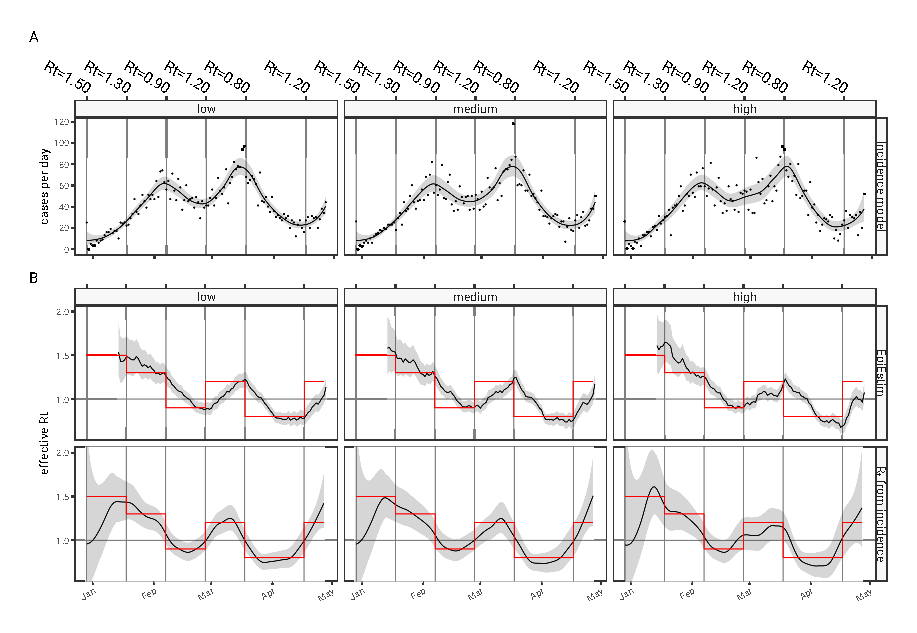
\includegraphics{fig/fig1-noise-qualitative}}
\caption{{\bf Instantaneous reproduction number estimates from a branching process model simulation.}
A qualitative comparison of instantaneous reproduction number estimates is shown. Panel A shows three case time series based on a single run of a branching process model parametrised with a stepped reproduction number time series (red lines in panel B) and infectivity profile as in \nameref{S1_Appendix} Fig S1. Case counts are shown as dots. A smoothed estimate of the cases per day as a line with shaded 95\% confidence intervals, based on a simple Poisson regression model. All three time series have on average 70\% case ascertainment, however the day to day variability of ascertainment is parametrised as a Beta distributed random variable, with ``low'', ``medium'' and ``high'' relating to the coefficient of variation of the Beta distribution (see \nameref{S1_Appendix} Table S1). Panel B shows estimates of the reproduction number based on the methods presented in this paper, and in the top row `EpiEstim` estimates derived from the data points in panel A are shown. In the middle row $R_t$ esimtates from a combination of GAM incidence model and the methods described in the paper. In the bottom row, $R_t$ estimates derived from a `Locfit' incidence model. In panel B the parametrised $R_t$ is shown as a solid red line and can be regarded as the ground truth for this single simulation run.}
\label{fig1}
\end{figure}

In the main validation scenario we used a window for `EpiEstim', `GAM' and `Locfit' of 14 days. We saw in Fig~\ref{fig1} that this results in the estimate of $R_t$ lagging the true value. This is quantified in Table~\ref{tab1} and Fig~S2 in the \nameref{S1_Appendix}. In the main analysis `EpiEstim' tends to produce an estimate delayed by 7 days and this lag is corrected by shifting the estimate in time before other metrics are calculated. In the first sensitivity analyses with a window of 7 days, a 4 day lag is observed for `EpiEstim', and in the second sensitivity analysis the metrics are calculated without correcting for lags.

\begin{table}[!ht]
\caption{{\bf Estimator delays in the validation scenarios}}
\centerline{\includegraphics{fig/tab1-lags}}
\label{tab1}
\end{table}

A quantification of the quality of the two estimation methods is shown in Fig~\ref{fig2} summarised from all 750 simulations, and corrected for estimator delays. In panel A the continuous ranked probability score is lower (better) for `$R_t$ GAM' and `$R_t$ Locfit' over all scenarios combined. In panel B the proportional difference between the true value and the median of the estimate probability (expressed as a percentage change) shows that the `EpiEstim` and `$R_t$ GAM' exhibit little bias, whereas `$R_t$ Locfit' demonstrates a tendency to underestimation, in this set of experiments. In Fig~\ref{fig2} panel C, the 50\% prediction interval width is smaller for `EpiEstim' and `$R_t$ GAM' demonstrating sharper, more confident, estimates than the predictions of `$R_t$ Locfit'. `$R_t$ Locfit' is the only method which has evidence of decreasing sharpness (increasing interval width - Fig~\ref{fig2} panel C) with increasing data noise. `EpiEstim' does not exhibit this change in sharpness with data noise and `$R_t$ GAM' only minimally. The low values of the probability of 50\% prediction coverage, as seen in panel D, which is ideally 0.5, implies that `EpiEstim` and `$R_t$ GAM' are over-confident in its predictions, `$R_t$ Locfit' on the other hand looks to be somewhat conservative, at least with more noisy data. The PIT Wasserstein metric in Fig~\ref{fig2} panel E, allows us to compare the calibration of the 2 methods on the same scale, one of which is over confident and the other being under confident. This suggests `$R_t$ Locfit' is better calibrated than `EpiEstim' or `$R_t$ GAM' (albeit in a different direction). Finally Fig~\ref{fig2} panel F shows the probability of misclassification at the threshold of $R_t=1$ which is similar for `EpiEstim' and `$R_t$ Locfit', but lower (better) for `$R_t$ GAM'. We also looked at how these metrics varied between scenarios (details in \nameref{S1_Appendix} Fig S3 and S4) and the breakdown largely follows the summary presented in Fig~\ref{fig2}, although `$R_t$ GAM' performs relatively poorly in scenario 3, and in scenario 5, which has relatively little variation compared to the others, calibration is better for `EpiEstim', and `$R_t$ GAM' appears overconfident.

\begin{figure}[!hb]
\centerline{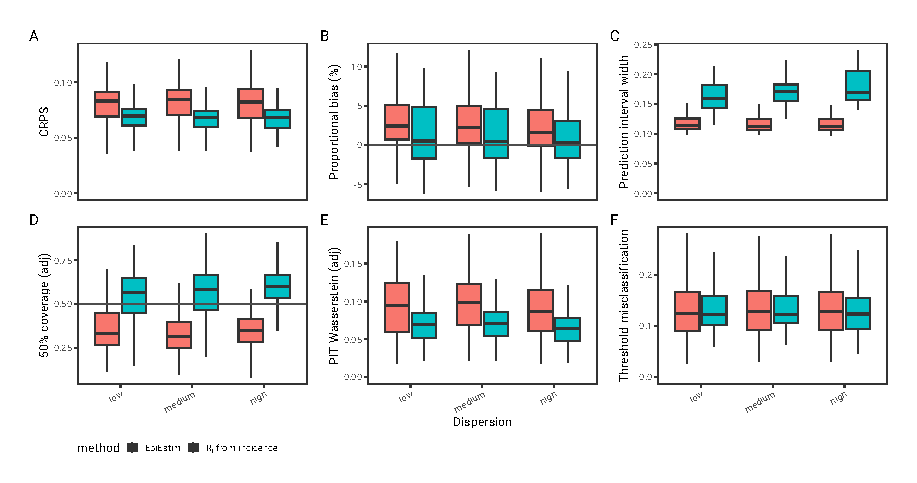
\includegraphics{fig/fig2-comparison}}
\caption{{\bf Quantitative comparison of $R_t$ estimation methods applied to 50 simulations of 5 scenarios at 3 levels of ascertainment noise.} The figure compares metrics describing the overall performance of the estimators. In Panel A is the continuous ranked probability score (CRPS) - lower is better; the average proportional bias (panel B) which characterise bias - lower is better; In panel C, the 50\% prediction interval width measures estimator sharpness, and lower is better if the estimator is unbiased and well calibrated. In Panel D the probability of 50\% coverage (ideal value is 0.5), and in Panel E the adjusted probability integral transform (PIT) Wasserstein metric (lower is better) are both measures of calibration. In Panel F a functional metric which quantifies the probability that an estimate is the wrong side of the cirtical threshold of $R_t=1$ desribes utility in decision making.}
\label{fig2}
\end{figure}

In the first sensitivity analysis (\nameref{S1_Appendix} Fig S5), the amount of data informing the $R_t$ estimates is reduced from 14 to 7 days, resulting in reduced certainty in both estimators. This changes the relative performance of the 2 methods as measured the the CRPS, which is now tends to favour `$R_t$ GAM' as the better overall estimator, despite continued bias, excess sharpness and mis-calibration. The certainty of `$R_t$ Locfit' has dropped to a low level and it has become excessively conservative in all but the high ascertainment noise scenarios (further details in \nameref{S1_Appendix}). This also slightly increases the probability of misclassification at the threshold of $R_t=1$ for `$R_t$ Locfit', although `$R_t$ GAM' still outperforms other methods on this more functional metric. In the second sensitivity analysis with no correction for lag (details in \nameref{S1_Appendix} Fig S6), `EpiEstim`, which is affected by lag, performs much less well in all metrics as the lag penalises all dimensions of the quality of the estimator, and this serves to highlight the importance of addressing lag before comparing the bias and calibration of estimators.

\section*{Discussion}

In this paper we describe a mathematical method for deriving an estimate of the effective reproduction number ($R_t$) from modelled estimates of disease incidence, that incorporates uncertainty from both incidence model and infectivity profile. Using a two stage process it allows for a flexible approach to incidence modelling that allows us to address many issues, such as right truncation, anomalies, missing data, or temporally aggregated data \cite{nash2023}, before using this to estimate $R_t$. At the same time our method propagates uncertainty from incidence models and infectivity profiles to $R_t$ estimates appropriately. We provide evidence that when combined with basic incidence models, our method produces $R_t$ estimates that are comparable to the de-facto standard algorithm implemented in `EpiEstim' \cite{thompson2019}, when assessed against synthetic outbreak data. 

There is a similar approach to deriving $R_t$ from modelled incidence described by Gressani et al.\cite{gressani2022}. It assumes a specific formulation for the incidence model as a negative binomial distribution estimated with P-splines in a Bayesian framework with Laplace approximations. This encouragingly also gives log normally distributed estimates for $R_t$, but its methodology is predicated on the specifics of the P-spline posterior vector and it does not incorporate infectivity profile uncertainty.

By comparison the approach in this paper is only loosely coupled to the incidence estimate framework and so can be applied to any incidence model that produces a time varying log-normally distributed incidence estimate. This includes a broad family of Poisson and negative binomial regression models \cite{nelder1972,loader1999,hastie2017}, or latent Gaussian models \cite{rue2009} using logarithmic link functions, and is agnostic to the formulation of those models. The incidence models could for example include covariates such as day of week effects, incorporate change points, or include spatial dimensions without affecting the derivation of the reproduction number estimates.

In terms of infectivity profile, our method is robust to distributions with zero or negative time intervals between index and secondary observations. It could therefore be used with directly observed real world serial interval distributions \cite{park2021} and delayed case counts as proxies for infectivity profile and infection incidence, which are necessarily inferred quantities; this is explored further in the `ggoutbreak' package documentation (\url{https://ai4ci.github.io/ggoutbreak/}). Our method does not specifically address important questions arising from ascertainment bias, or right truncation of observed incidence  \cite{abbott2020,abbott2024}, however when input incidence models have been adapted to right censored data our method can be used to derive an $R_t$ estimate (see package documentation for an example).

The validation comparison here combines one very simple statistical model of incidence `$R_t$ Locfit', and one more sophisticated model `$R_t$ GAM', with our method to derive $R_t$ estimates, and compares them to estimates produced direct from the count data by `EpiEstim'. This shows that the combination of incidence models and our $R_t$ derivation, produces estimates similar to `EpiEstim`. We have not formally tested the statistical significance of the differences because they are based on a large number of observations, and even tiny differences will be statistically significant. We pragmatically chose to simulate using a set of 5 step functions for $R_t$ parametrisation, which we expect to be relatively challenging for both `EpiEstim' and the statistical models for incidence we used here. The relative performance between the methods varies with the exact details of the test scenario (see \nameref{S1_Appendix} Fig S6). A more realistic smooth $R_t$ parametrisation time series has been performed and both methods perform better in such scenarios, so we consider our simulations to be worst case. There are some scenarios in which `EpiEstim' performs better and others in which incidence model derived estimates performs better. In comparing the models we ignored the first 20 $R_t$ estimates which are unstable in `EpiEstim` and very uncertain in `$R_t$ Locfit', this will tend to discriminate against `$R_t$ GAM' which seems to be much more accurate in the first 20 days.

Our method is not a replacement for `EpiEstim' as it requires an incidence model derived from count data, rather than directly using data, and any comparison is looking at both the incidence model quality and the method for deriving $R_t$. This must be taken into account when interpreting the validation section of this paper. By picking two statistical models for incidence with different characteristics, to which to apply our method for estimating $R_t$, we hope to demonstrate that the combinations are not obviously inferior to `EpiEstim'. If we had used different incidence models, the overall $R_t$ estimate may have very different characteristics. The choice of best estimator is subjective as it depends on whether it is more important to have an estimator that minimises the risk of a misclassification between a growing or shrinking epidemic, or whether a more accurate representation of uncertainty is required. Estimates of later time points are also arguably more important in managing an epidemic.

Notwithstanding these limitations in validation, we argue our method for deriving $R_t$ from log-normally modelled incidence estimates, which are commonly produced by statistical modelling frameworks, is a useful adjunct to the range of tools available for monitoring an epidemic. It is relatively quick and deterministic, and is flexible enough to be combined with a wide range of temporal incidence modelling techniques, which can for example account for reporting delays, ascertainment bias, temporally aggregated data, and noisy missing data. 

\nolinenumbers

\bibliography{refs}

\section*{Funding}

RC and LD are funded by UK Research and Innovation AI programme of the Engineering and Physical Sciences Research Council, AI for Collective Intelligence Research Hub (EPSRC grant EP/Y028392/1;  \url{https://gtr.ukri.org/projects?ref=EP%2FY028392%2F1}). RC and LD are affiliated with the JUNIPER partnership funded by the Medical Research Council (MRC grant MR/X018598/1; \url{https://www.ukri.org/councils/mrc/}). The views expressed are those of the authors.

\section*{Competing interests}

The authors have no competing interests to declare.

\section*{Author contributions}

RC and LD generated the research questions. RC performed the mathematical analysis and simulations, and created the supporting software package. RC and LD provided validation of the methods. LD provided supervision of the research. RC developed the first draft of the manuscript. RC and LD contributed to the final editing of the manuscript and its revision for publication and had responsibility for the decision to publish.

\subsection*{Use of large language models}

We acknowledge the input of the large language model QWEN3-235B-A22B-2507, principally in refining the mathematical methods in this paper. All methods were conceptualised by the authors, but QWEN3 was used to improve the handling of estimate covariance and the assessment of the bias when assuming independence (\nameref{S3_Appendix}). QWEN3 was also used to improve the formatting of the mathematical notation and identify inconsistencies. There was no use of LLMs in generating the final narrative of this paper, or in validation of the methods. The reference implementations of these methods was written without the use of LLMs, except for the code responsible for the generation of synthetic variance-covariance matrices. All mathematical and code generated by QWEN3 was rigorously reviewed and tested by the authors. Discussion history is available from the corresponding author on request.

\section*{Data and code availability}

All data and code used for running experiments, model fitting, and plotting is available on a GitHub repository at \url{https://ai4ci.github.io/ggoutbreak-paper/}. The methods described here are implemented in the form of an R package to support the estimation of epidemiological parameters and it is deployed on the AI4CI r-universe (\url{https://ai4ci.r-universe.dev/ggoutbreak}). We have also used Zenodo to assign a DOI to the repository: doi:10.5281/zenodo.7691196.

\section*{Supporting information}

% Include only the SI item label in the paragraph heading. Use the \nameref{label} command to cite SI items in the text.

\paragraph*{S1 Appendix.}
\label{S1_Appendix}
{\bf Simulation for validating Rt estimates, additional results and sensitivity analyses} Methodological details of simulation set up for validating the performance of $R_t$ estimators presented in the main paper, additional figures and detailed results from the sensitivity analyses.

\paragraph*{S2 Appendix.}
\label{S2_Appendix}
{\bf Metrics for evaluating the quality of probabilistic estimators.} Methodological details of performance metrics used for validating the performance of $R_t$ estimators presented in the main paper.

\paragraph*{S3 Appendix.}
\label{S3_Appendix}
{\bf Bias in $ R_t $ Estimation Under Independence and Heuristics for Risk Assessment.} This appendix provides bounding of bias in $R_t$ estimates under the assumption of independence of incidence estimates, and derives of metrics to assess whether the assumption of independence is valid.

\end{document}

